\section{Kinematic ages}
\subsection{Calculating velocity dispersions}
\label{sec:velocity_dispersion}

A kinematic age can be calculated from the velocity dispersion, \ie\ standard
deviation, of a group of stars.
These velocity dispersions can then be converted into an age using an AVR
\citep[\eg][]{holmberg2009, yu2018}.
Kinematic ages represent the {\it average age} of a group of stars and are
most informative when stars are grouped by age.
If a group of stars have similar ages, their kinematic age will be close
the age of each individual.
On the other hand, the kinematic age of a group with large age variance will
not provide much information about the ages of individual stars.
Velocity distributions themselves do not reveal whether a group of stars have
similar or different ages, since either case the velocities are
Gaussian-distributed.
Fortunately however, we can group \kepler\ stars by age using the implicit
assumption that underpins gyrochronology: that stars with the same rotation
period and color are the same age.
% We discuss the implications of this assumption and cases where it doesn't
% apply in the Discussion of this paper (section \ref{sec:discussion}).

In this paper, we use the kinematic ages published in \citet{lu2021}.
In that work, the kinematic age of each star in our sample was calculated by
placing it in a bin with other stars with similar rotation periods, effective
temperatures, absolute Gaia magnitudes and Rossby numbers.
The kinematic age of each star was estimated by calculating the velocity
dispersions of stars with these similar parameters, then using an AVR to
calculate a corresponding age \citep{yu2019}.
The bin size was optimized using a number of Kepler stars with asteroseismic
ages.

We used the \citet{yu2018} AVR to convert velocity dispersion to age.
This relation was calibrated using the ages and velocities of red clump stars.
They divided their sample into metal rich and poor subsets, and calibrated
separate AVRs for each, plus a global AVR.
Their AVR is a power law:
\begin{equation}
    \sigma_{vz} = \alpha t ^\beta,
\end{equation}
where $\alpha$ and $\beta$ take values (6.38, 0.578) for metal rich stars
(3.89, 1.01) for metal poor stars, and (5.47, 0.765) for all stars.

We used 1.5$\times$ the Median Absolute Deviation (MAD) of velocities, which
is a robust approximation to the standard deviation and is less sensitive to
outliers.
Velocity outliers could be binary stars or could be generated by
underestimated parallax or proper motion uncertainties.

Figure \ref{fig:kin_and_clusters} displays the data we used to calibrate our
gyrochronology model in \prot-\teff\ space.
Kepler field stars are shown as small points, and cluster stars are larger
points with black outlines.
Points are colored by either their kinematic ages or cluster ages.
The left- and right-hand panels have a linear and logarithmic y-axis,
respectively.

\begin{figure}
\caption{
    The calibration data.
Kepler field stars are shown as small points, and cluster stars are larger
points with black outlines.
Points are colored by either their kinematic ages or cluster ages.
The left- and right-hand panels have a linear and logarithmic y-axis,
respectively.
}
  \centering 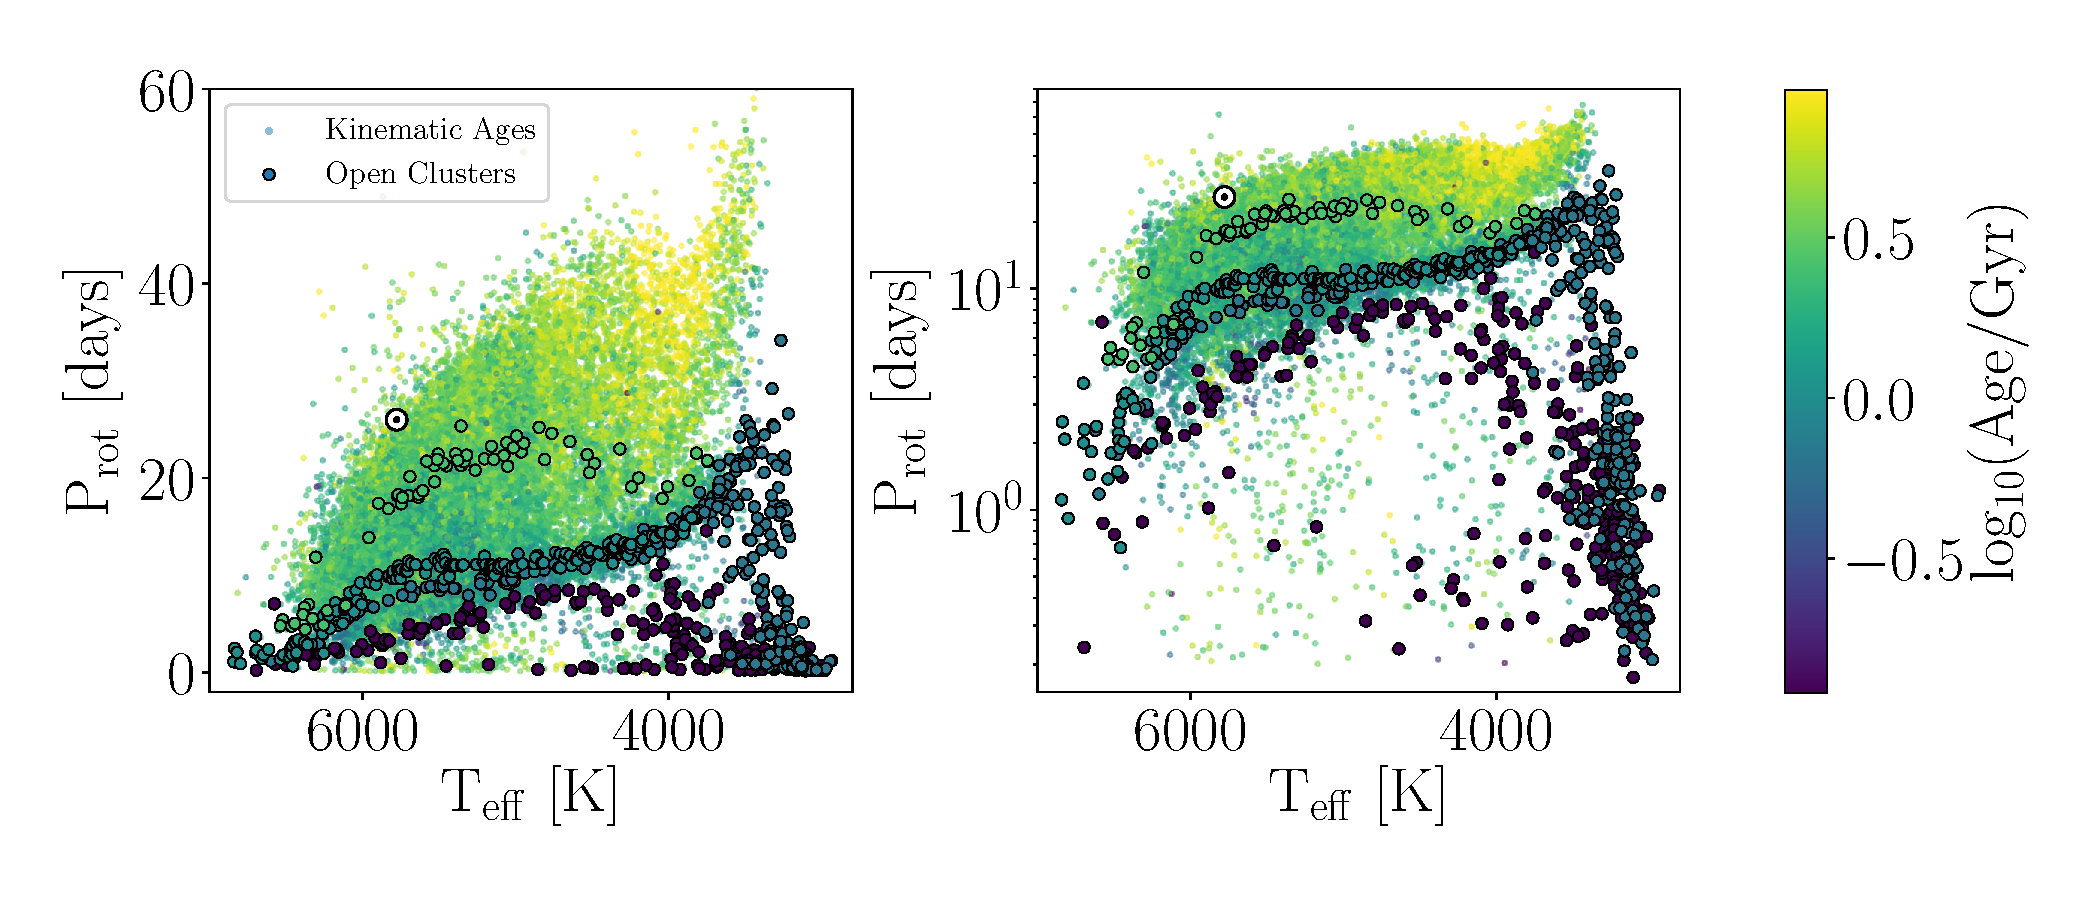
\includegraphics[width=1\textwidth]{kin_and_clusters_log_lin}
\end{figure}
